
\section{Example Simulation: Cosmic Reionization by Stellar Sources}
\label{sec:example_simulation}

To illustrate the application of our radiation hydrodynamic cosmological code we
simulate hydrogen reionization due to stellar sources in a comoving volume of {\bf (80 Mpc)$^3$ with a grid
resolution of $3200^3$} and the same number of dark matter particles {\bf (this is the RHD simulation referred to above.)} This yields a comoving spatial resolution of 25 kpc and
dark matter particle mass of $4.8 \times 10^5 M_{\odot}$. This resolution yields a dark matter halo mass function that
is complete down to $M_h = 10^8 M_{\odot}$, which is by design, since this is the mass scale below 
which gas cooling becomes inefficient {\bf (but see, however, \cite{Wise2014}.) The box is large enough to contain the rare, luminous galaxies at the bright end of the high-z galaxy luminosity function (Norman et al., in prep.)}

We simulate a $\Lambda$CDM cosmological model with the following parameters: 
$\Omega_{\Lambda} = 0.73$, $\Omega_m = 0.27$, $\Omega_b = 0.047$, 
$h = 0.7$, $\sigma_8 = 0.82$, $n_s = 0.95$, where these are, respectively, the fraction of the 
closure density at the present epoch in vacuum energy, matter, baryons;
the Hubble contant in units of 100 km/s/Mpc; the power spectrum normalization; 
and the slope of the scalar fluctuations of the primordial power spectrum. These are
consistent with the 7-year WMAP measurements \cite{WMAP7}. A Gaussian random
field is initialized at z=99 using the {\em Enzo} initial conditions generator {\em init} 
using the Eisenstein \& Hu (1999) fits to the transfer functions. The star formation efficiency
parameter $f_*$ is adjusted to match the observed star formation rate density in the interval $6 \leq z \leq 10$ from
Bouwens et al. (2011).  {\bf Further details of the simulation input parameters and assumptions are described in \cite{So2014} as they are identical to the smaller 20 Mpc box simulation analyzed there.
The simulation was run to a stopping redshift of z = 5.5 and consumed 38 Million core-hrs running on 31,264 cores of the Cray XT5 system {\em Jaguar} operated by the 
National Center for Computational Science at ORNL. }

{\bf Fig. \ref{fig:simulation} shows slices of gas density and temperature at z=6.5 through the simulation volume. Reionization begins at $z \approx 14$ with the first luminous sources inflating isolated HII regions, and completes at 
$z \approx 5.8$ after the HII regions merge and overlap. The HII regions are roughly spherical until they begin to merge, which is
indicative of the photon budget for reionization being dominated by fewer, more luminous sources, as opposed to numerous low luminosity sources \cite{Zahn07}. In general appearance they are not dissimilar to the post-processing results of \cite{Iliev06,TracCen2007}.
An inspection of the temperature projections shows photoionized gas in green, with smaller pockets of shock heated gas near the centers of HII regions, resulting from thermal feedback from supernovae. This simulation is discussed in detail in Norman et al. 2014, {\em in preparation}.}

\begin{figure}[t]
\centerline{\hfill
  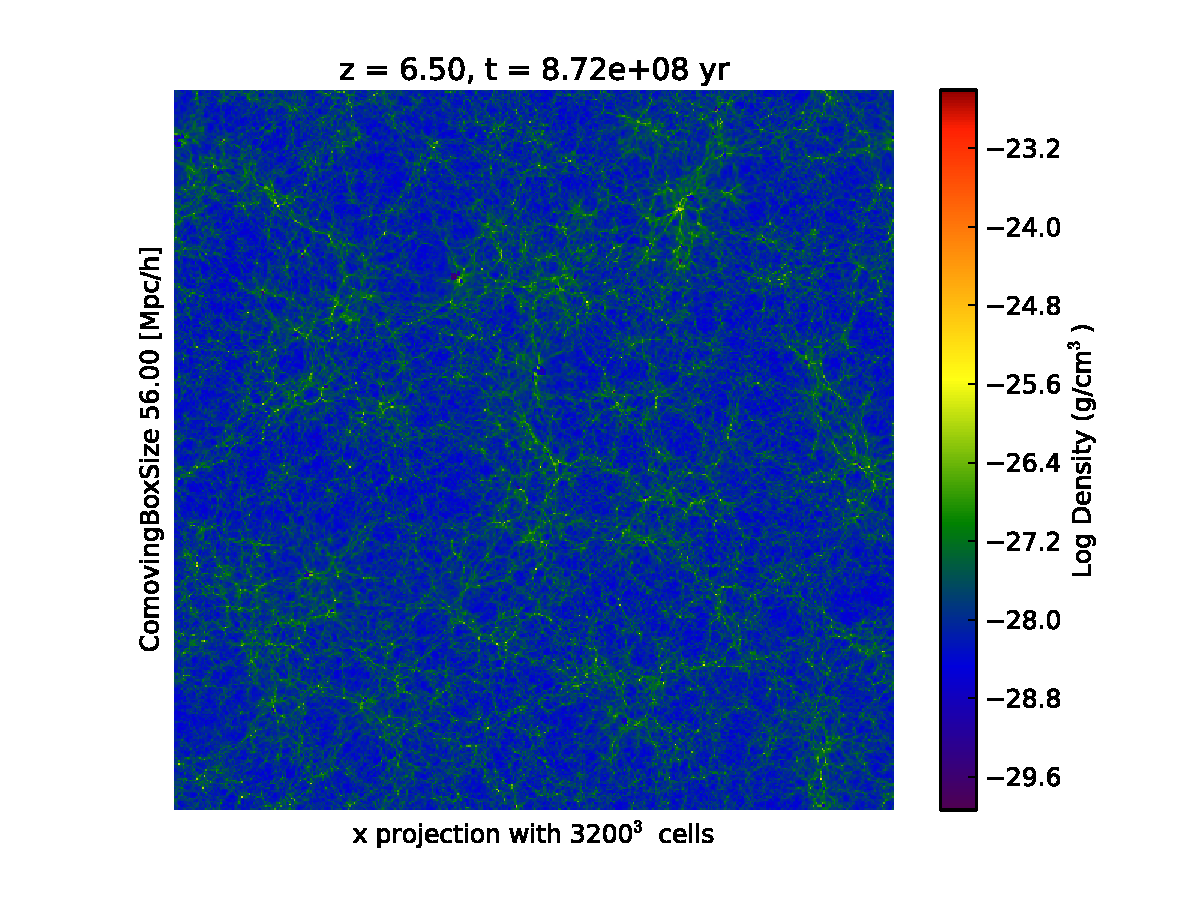
\includegraphics[scale=0.75, trim=0.5cm 0.5cm 0.5cm 0.5cm]{slice_Density_x_HD14901.pdf}
  \hfill}
\centerline{\hfill
  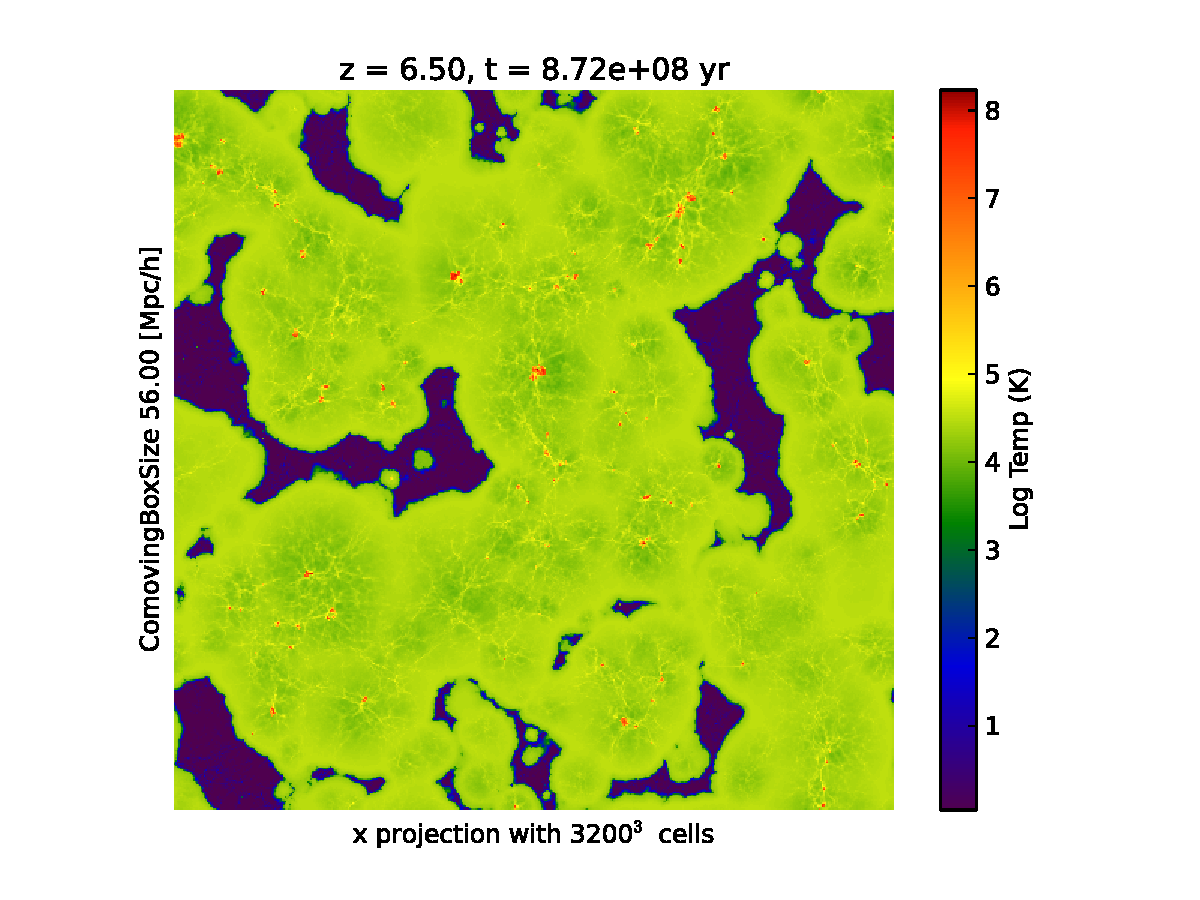
\includegraphics[scale=0.75, trim=0.5cm 0.5cm 0.5cm 0.5cm]{slice_Temperature_x_HD14901.pdf}
  \hfill}
  \caption{Application of the numerical methods described in this paper to cosmological hydrogen reionization. Shown are slices of gas density and temperature at z=6.5 through a (80 Mpc)$^3$ simulation volume resolved with mesh of $3200^3$ Eulerian cells and $3200^3$ dark matter particles.}
  \label{fig:simulation}
\end{figure}
